\documentclass[12pt, a4paper]{article}
% Packages: 
\usepackage[utf8]{inputenc}
\usepackage[T1]{fontenc}
\usepackage[polish]{babel}
\usepackage[utf8]{inputenc}
\usepackage{lmodern}
\usepackage{graphicx}
\usepackage{indentfirst}
\usepackage{fancyhdr}
%------------------------------------
% Style config etc.:
\selectlanguage{polish}
\brokenpenalty=1000
\clubpenalty=1000
\widowpenalty=1000    
\pagestyle{fancy}
\fancyhead{}
\fancyfoot{}
\rfoot{\thepage}
\lfoot{}
\lhead{}
\rhead{}
\renewcommand{\headrulewidth}{1pt}
\renewcommand{\footrulewidth}{1pt}
%--------------------
\title{Integracja mongo DB z mongo-express przy pomocy Docker'a oraz Docker-compose}
\author{Marian Dorosz}
\date{23.03.2022}

\begin{document}

\maketitle
\newpage

\tableofcontents
\newpage

\listoffigures
\newpage

\section{Pobieranie obrazów z DockerHub'a}
    Pierwszym krokiem jest pobranie obrazów kontenerów z DockerHub'a. Aby to zrobić należy skorzystać z polecenia \textbf{docker pull nazwa obrazu}. W przypadku obu obrazów należy skorzystać z tego samego polecenia, więc poniżej pojawi się przykład tylko dla obrazu mongo DB.
    \begin{figure}[!h]
        \centering
        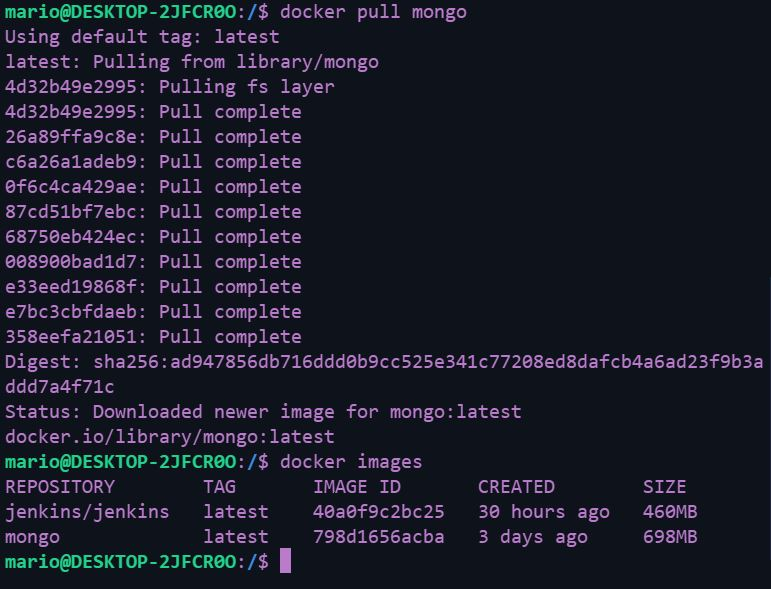
\includegraphics[width=\textwidth]{docker_pull_mongoDB.JPG}
        \caption{Pobieranie obrazu mongo DB}
        \label{fig:pobieranie_mongoDB}
    \end{figure}
    \\
    Wykorzystanie ww. polecenia - \textbf{docker pull mongo} spowoduje, że na nasz komputer zostanie pobrany obraz kontenera aplikacji mongo DB. 
    
\section{Konstruowanie pliku docker-compose.yaml}
    \subsection{Do czego służą pliki typu docker-compose.yaml?}
        Piki \textbf{docker-compose.yaml} usprawniają tworzenie kontenerów, gdyż powstały do tworzenia dużej ilości kontenerów małym nakładem pracy. Dodatkowo infrastruktura aplikacji utworzona w tych plikach staje się szablonem, przez co taki plik możemy w zasadzie uruchomić na każdym komputerze, który posiada Docker'a i dostęp do internetu. Gdy posiadamy gotowy plik, wystarczy skorzystać z polecenia - \textbf{docker-compose -f (nazwa pliku).yaml up}. Polecenie to spowoduje, że Docker utworzy kontenery zgodnie z konfiguracją zawartą w pliku.  
    \subsection{Analiza pliku Compose, potrzebnego do zintegrowania mongo DB z mongo-express}
        \begin{figure}[!h]
            \centering
            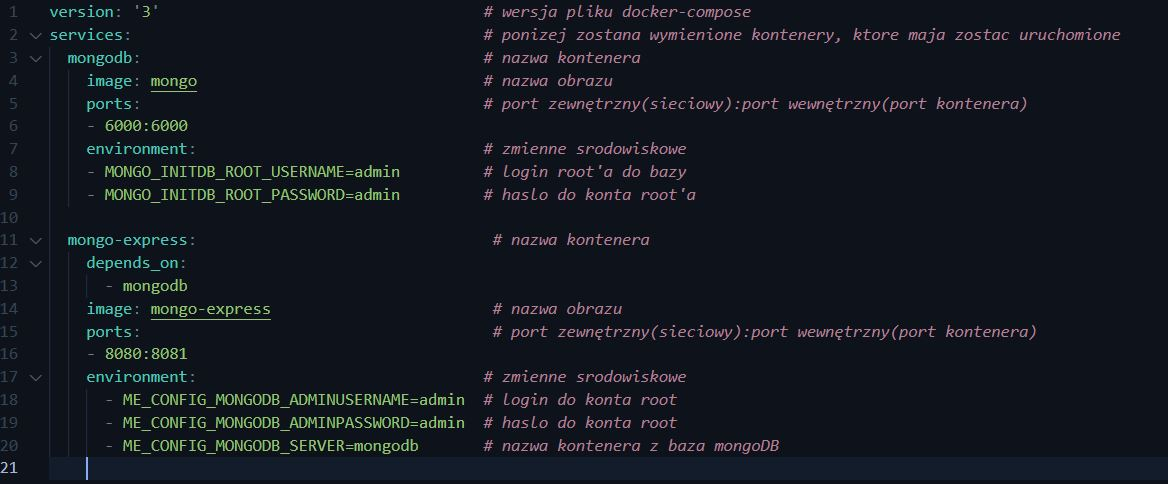
\includegraphics[width=\textwidth]{docker-compose.JPG}
            \caption{Kod potrzebnego pliku}
            \label{fig:kod_docker-compose}
        \end{figure}
        \paragraph{Wersja pliku docker-compose} Parametr \textbf{version:'3'} jest informacją, jakiej wersji jest plik  Compose, który tworzymy. Wersja 3 została stworzona aby była kompatybilna w docker-compose oraz docker swarm.
        \paragraph{Nazwa kontenera} Pierwszym parametrem kontenera, który ustawia się w pliku Compose jest jego nazwa. Aby utworzyć kontener o zadanej przez nas nazwie wystarczy wpisać w pliku \textbf{nazwa\_kontenera:}. Po uzupełnieniu nazwy można konfigurować dodatkowe parametry kontenera.
        \paragraph{Nazwa obrazu} Parametrem \textbf{image: nazwa obrazu} ustalamy jaki obraz będzie wykorzystany do utworzenia kontenera.
        \paragraph{Port zewnętrzny(sieciowy):port wewnętrzny(port kontenera)} Parametrem \textbf{Ports: port zewnętrzny:port wewnętrzny} ustawiamy porty zewnętrzne (TCP) oraz wewnętrzne (porty na których nasłuchuje kontener). Mapowanie portów powstało, aby umożliwić łączenie się z aplikacją uruchomioną w kontenerze z poziomu komputera.
        \paragraph{Zmienne środowiskowe} Parametr \textbf{environment} pozwala na uruchomienie kontenera z dodatkowymi opcjami konfiguracyjnymi, które nie są elementami samego docker'a, lecz są dodatkowymi konfigurowalnymi parametrami aplikacji. Przykładowo: w przypadku mongo DB jest to skonfigurowanie loginu i hasła root'a dla systemu bazodanowego.
        \paragraph{Depends on} Ten parametr spowoduje, że kontener z aplikacją mongo-express nie powstanie dopóki nie zostanie uruchomiony kontener mongo DB.
    \subsection{Uruchomienie pliku Compose}
        Pliki typu Compose uruchamia się wcześniej wspomnianym: 
        \\
        \textbf{docker-compose -f (nazwa pliku).yaml up}. 
        \subsubsection{Wynik uruchomienia pliku}
            \begin{figure}[!h]
                \centering
                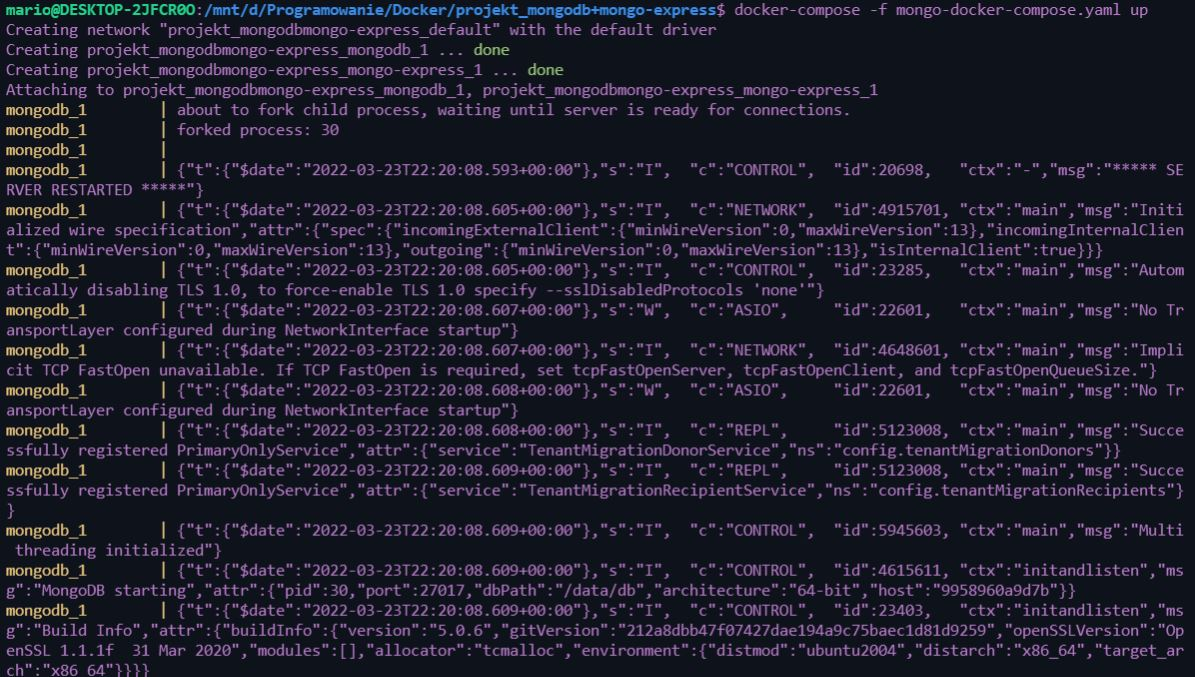
\includegraphics[width=\textwidth]{docker-compose-f.JPG}
                \caption{Wynik uruchomienia stworzonego pliku docker-compose}
                \label{fig:docker_compose_f}
            \end{figure}
            Uruchomienie utworzonego wcześniej pliku docker-compose spowoduje utworzenie dwóch kontenerów, przechowujących aplikacje mongo DB oraz mongo-express. Z obiema aplikacjami można połączyć się z poziomu komputera, na którym je uruchomiono.
    \subsection{Test działania}
    \begin{figure}[!h]
        \centering
        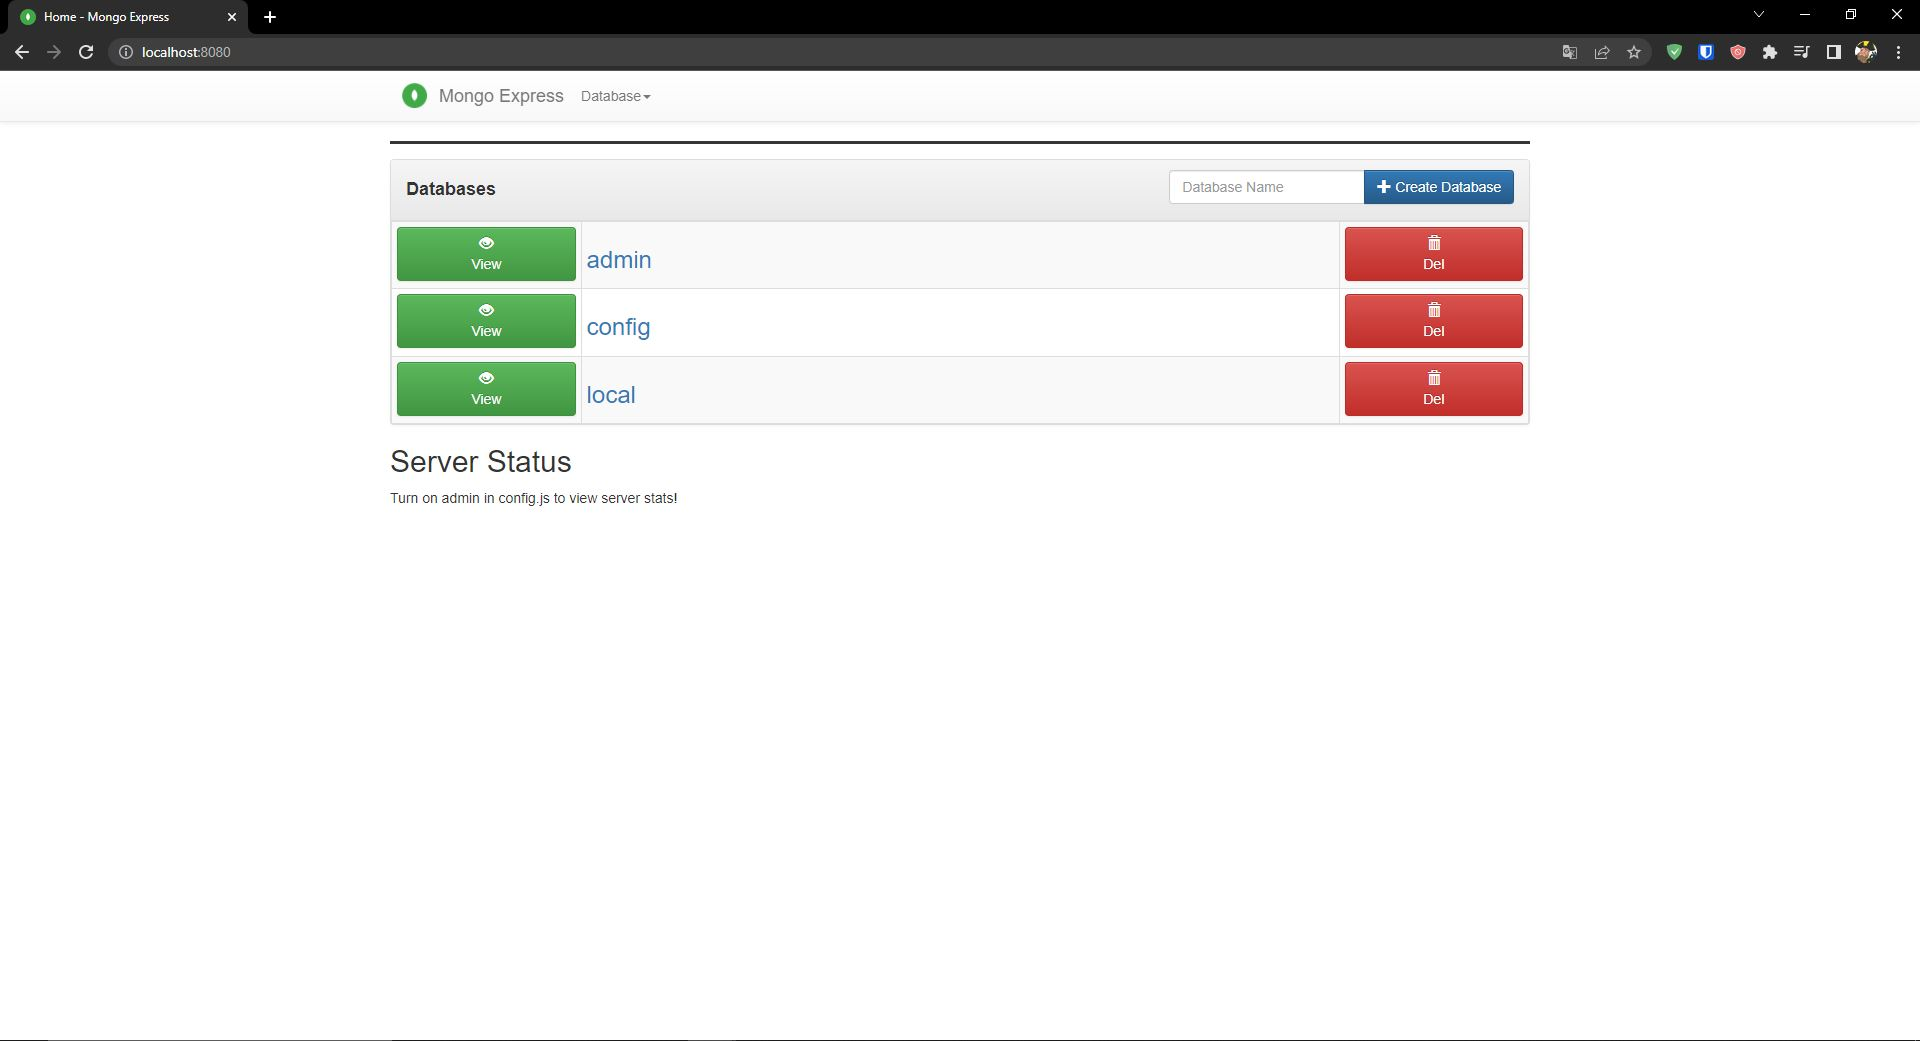
\includegraphics[width=\textwidth]{mongo-express.JPG}
        \caption{Działająca aplikacja mongo-express}
        \label{fig:mongo_express}
    \end{figure}
    Jak widać na powyższym zrzucie, z poziomu komputera można zalogować się do aplikacji mongo-express, która łączy się z mongo DB, a więc integracja obu systemów powiodła się. 
    \subsection{Cofanie efektów pliku docker-compose}
    \begin{figure}[!h]
        \centering
        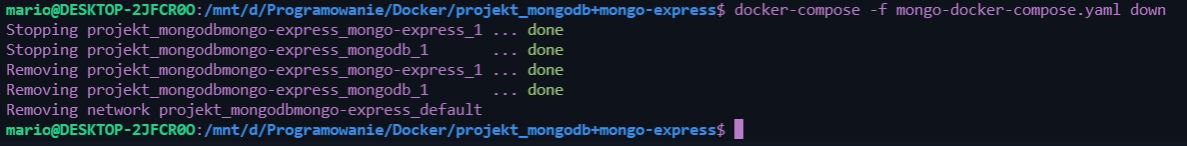
\includegraphics[width=\textwidth]{docker-compose-f-down.JPG}
        \caption{Cofanie efektów działania pliku docker-compose.yaml}
        \label{fig:docker_compose_down}
    \end{figure}
    Jak widać na powyższym zrzucie cofnięcie efektów działania pliku docker-compose jest bardzo proste. Wystarczy skorzystać z polecenia \textbf{docker-compose -f (nazwa pliku).yaml down}. Po wpisaniu polecenia docker automatycznie usunie wszystkie kontenery oraz sieć docker net, którą utworzył wcześniej.
\end{document}
